\chapter{実装}
\label{implementation}
本章では実装について述べる。

\newpage
\section{Rive Client}
\label{sec:riveclient}
\subsection{システムフロー}

このシステムが立ち上がるとまず始めにonCreate()が呼ばれ、初期化を行う。
その後onStartInput()メソッドが呼ばれコンテキストを取得する。
このコンテキストはデバイスの情報を取得する。
コンテキストを取得し次第、候補単語を取得する。
この候補単語はサーバーと通信した上で取得する。
これをユーザーが一つの操作を行うたびに繰り返す。
ここで言う一つの動作とは、キーボード上の一つの文字を押すことや、
候補の単語をタップすること、
あるいは文字をデリートすることも含まれる。
最終的にユーザーが入力を終了した場合にはonFinishInput()が呼ばれ、
今回のユーザが行った動作とコンテキストを紐付けサーバーに送信する。
通信が終わり次第onDestory()が呼ばれ本システムは終了する。

\begin{figure}[htbp]
  \begin{center}
    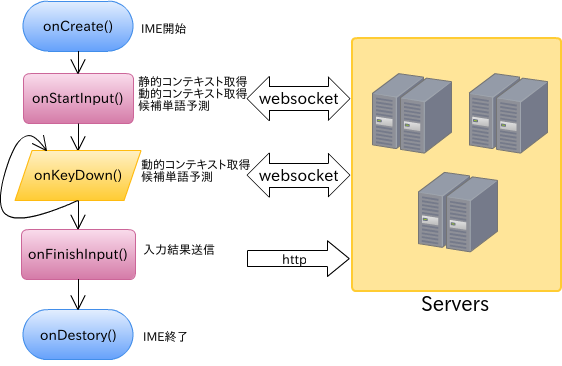
\includegraphics[width=14cm,bb=0 0 562 366]{images/clientflow}
  \end{center}
  \caption{Rive Clientフローイメージ}
  \label{fig:clientflow}
\end{figure}

\subsection{コンテキスト取得}

取得するコンテキストについては\ref{sec:getcontext}項を参照。
コンテキストはユーザーに入力してもらえるものは入力してもらう。
またデバイスで取得可能なものを全て取得し、推薦システムに使う。

\section{Rive Server}
\subsection{システム構成}

サーバーの中身は大きくRoutting Server,beforeRules,afterRules,Jubatusの
4つを実装した。
それぞれ候補単語の計算手法が異なるため此のような分割になっている。
\begin{figure}[htbp]
  \begin{center}
    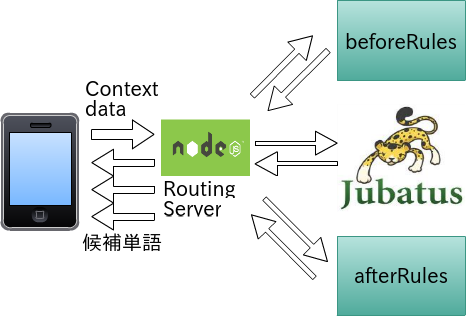
\includegraphics[width=14cm,bb=0 0 466 316]{images/riveserver.png}
  \end{center}
  \caption{Rive Server概要図}
  \label{fig:riveserver}
\end{figure}

\subsection{Routing Server}
このサーバーはふたとおりの役割を持っている。
一つはデバイスから受け取ったコンテキストデータを
beforeRules,Jubatus,afterRulesの3つの計算エンジンに振り分け送信する役割である。
もうひとつは受け取ったデータを受け取り次第、デバイスに送信する役割である。

\subsection{beforeRules}
このエンジンはコンテキストデータが送られてきた際に、
一定のルールに基づいているものをまとめている。
このルールは著者?開発者?がよく使われる単語を推測し実装した。
例えば、Twitter\cite{Twitter}クライアントに入力を行っている(行おうとしている)
場合に「なう」「@」の候補単語を返すようになっている。

\subsection{Jubatus}
このエンジンについては第\ref{sec:jubatus}項参照。

\subsection{afterRules}
このエンジンはbeforeRulesより重要度が低く、
また計算に時間がかかるものを推測して実装した。
例えば、最寄り駅をクエリとしてその駅を通っている電車の線を
その場でWEBから検索し推薦単語として返すことができる。

\section{Rive Analytics}
このシステムはRive Client\ref{sec:riveclient}でのプロセスの終わりに
送られてくるデータを受信し、解析するシステムである。
開発者はこのシステムを使用することによって、新しい機能の有用性などを
確かめることができる。

\subsection{指標値}
\begin{itemize}
  \item CPI(click per input)
    入力がどれだけどうか
  \item CPI
  \item CPI
\end{itemize}

\section{Rive BatchProcessing}
このシステムは定期的に処理を行うものを管理し実行している。

\section{Rive WebService}
このシステムはインターネット上で閲覧可能なホームページである。
Riveシステムを試用することができる。

